\documentclass[%
sor,
 jor,
 amsmath,amssymb,
 reprint,
longbibliography,
]{revtex4-2}
\usepackage{float}
\usepackage{caption}
\usepackage{empheq, amssymb, amsfonts}
\usepackage{siunitx}
\usepackage{graphicx}
\usepackage{circuitikz}
\usepackage{url}
\usepackage{hyperref}

\begin{document}
\title{PH3244\\Experiment - 5\\ The Cornus method of determining the elastic constants of a transparent material}
\author{Aumshree P. Shah\\20231059}
\altaffiliation{\color{red}aumshree.pinkalbenshah@students.iiserpune.ac.in}
\date{\today}
\begin{abstract}
In this experiment, we use Cornu’s method to determine the Young's moduls and Possion's ratio of a given acryllic slab.
\centering
\end{abstract}
\maketitle
\tableofcontents
\hfill
\newpage
\newpage\null\thispagestyle{empty}\newpage
\section{Theory and Procedure}
		\subsection{Theory\footnote{Please refer to [\cite{ph3244repo}] for a full examination of theory, only the important results will be discussed here.}}
	The radius of curvature of plano convex lens $R_0$ is given by:
		\begin{equation}
			R_0 = \frac{d_n^2}{4n\lambda}
		\end{equation}
		where the $d_n^2$ is the diameter of $n^{\text{th}}$ fringe, $\lambda$ is the wavelength used. The $d_n^{'2} \text{ and } d_n^{''2}$ along with $d_n^2$ can be seen properly in FIG - 1. 
	\begin{figure}[H]
	\begin{center}
		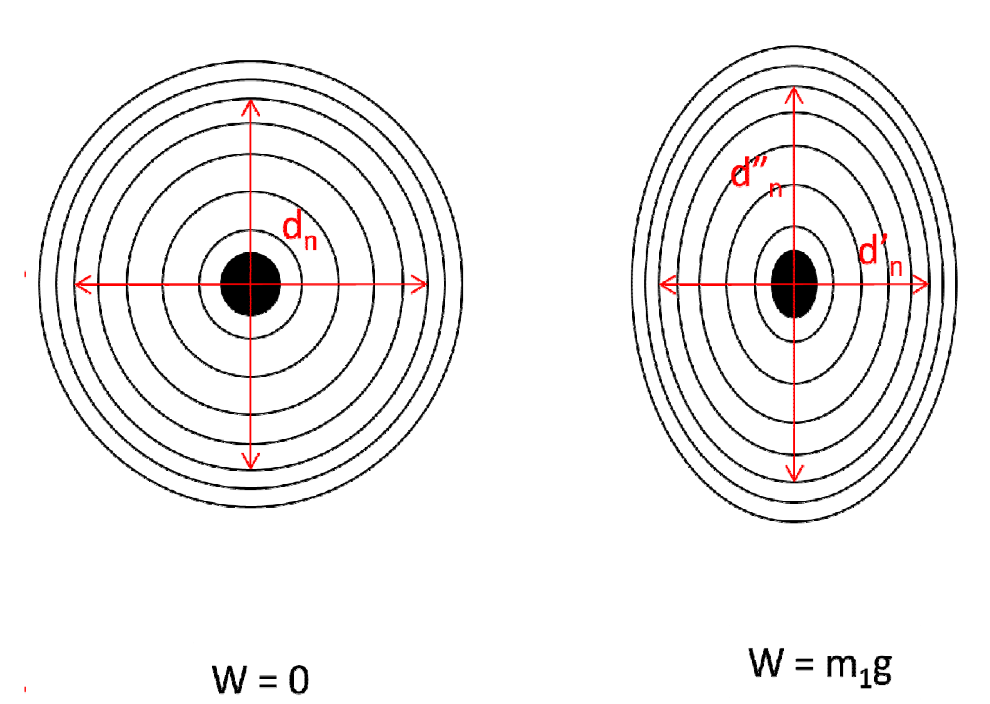
\includegraphics[width=0.5\linewidth]{fig1}
		\caption{Newton rings with and without bending shown, respectively, in the left and right panel.}
	\end{center}
	\end{figure}
	The Young's moduls ($Y$) and the Possion's ratio ($\zeta$) are calculated by:
		\begin{equation}
			Y = \frac {12m_1gLR_1} {wh^3}
		\end{equation}
		\begin{equation}
			\zeta = \frac {R_1}{ R_2}
		\end{equation}
	
	Here $m_1$ is the mass on each side of the bar, $g$ is the gravitational acceleration, $L$ is the length of the beam from the pivot to a end, $w$ and $h$ are width and height of the road respectively and can be seen from FIG - 2.
	
	\begin{figure}[H]
	\begin{center}
		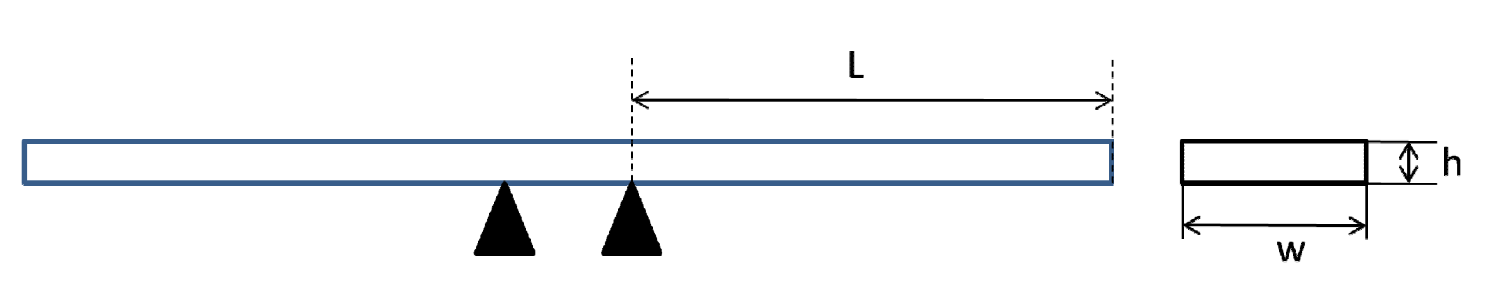
\includegraphics[width=1\linewidth]{fig2}
		\caption{Side views (the unloaded condition) of the beam whose elastic constants have to be determined. The beam  is supported on two triangular pegs (black triangular shape objects in the figure) }
	\end{center}
	\end{figure}
	
		Here $R_1$ and $R_2$ are obtained from the equations:
		 \begin{equation}
			 \frac 1 R_1 = 4n\lambda \left( \frac 1 {d_n^{'2}}  - \frac 1 {d_n^{2}} \right)
		 	 \end{equation}
	 \begin{equation}
			 \frac 1 R_2 = 4n\lambda \left( \frac 1 {d_n^{''2}}  - \frac 1 {d_n^{2}} \right)
		 	 \end{equation}

			 and are two differnet radius of curvature which can be seen from FIG - 3.
	
	\begin{figure}[H]
	\begin{center}
		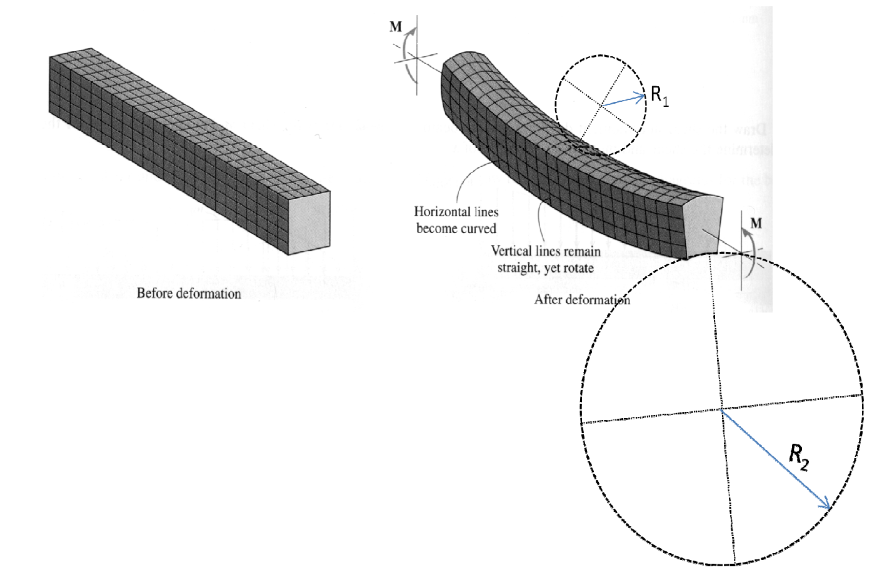
\includegraphics[width=0.6\linewidth]{fig3}
		\caption{Longitudinal bending ($R_1$) of a bean resulting in small lateral bending ($R_2$)}
	\end{center}
	\end{figure}

	\subsection{Procedure \footnote{Refer to the manual [\cite{ph3244repo}] for a look at procedure.}}

	From Equation - 1, 4 and 5, we can determine the values of $R_0$, $R_1$ and $R_2$ from the slope obtained by plotting the graph of $n$ vs different values form those radius of curvatures, form Equation - 2 and 3 we can determine what Youngs modulus and Possion's ratio of the given material is.





\section{Observation}
\subsubsection{Slab parameters and other values\footnote{The least count is to be interpreted from the significant figures written}}
\begin{align*}
	w &= 41\si{\mm}\\
    l &= 125\si{\mm}\\
    h &= 3.7\si{\mm}\\
    g &= 9.8*10^3 \si{\mm\per\second^2}\\
    \lambda &= 589 * 10^{-6}\si{\mm}
\end{align*}
\subsubsection{Fringe Readings\footnote{M.S. Stands for Main Scale Readings and C.S. Stands for Circulat Scale Readings}}
\begin{table}[H]
    \centering
    \begin{minipage}[t]{0.48\textwidth}
        \centering
\begin{tabular}{|c|c|c|c|}
\hline
\multicolumn{2}{|c|}{Left} & \multicolumn{2}{c|}{Right}\\
\hline
M.S. & C.S. & M.S. & C.S. \\
\hline
12.5 & 19 & 13.5 & 41 \\
12.5 & 9  & 13.5 & 49 \\
12.5 & 0  & 14.0 & 19 \\
13.0 & 43 & 14.0 & 26 \\
13.0 & 35 & 14.0 & 34 \\
13.0 & 29 & 14.0 & 44 \\
13.0 & 24 & 14.0 & 44 \\
\hline
\end{tabular}
\caption{Readings for $m_1=0$g.}

            \end{minipage}% <--- The '%' prevents a space that could cause a line break
    \hfill % Adds horizontal space between the minipages
    \begin{minipage}[t]{0.48\textwidth}
        \centering
\begin{tabular}{|c|c|c|c|c|c|c|c|}
\hline
\multicolumn{2}{|c|}{Left} & \multicolumn{2}{c|}{Right}  & \multicolumn{2}{c|}{Top} & \multicolumn{2}{c|}{Bottom}  \\
\hline
M.S. & C.S. & M.S. & C.S. & M.S. & C.S. & M.S. & C.S. \\ 
\hline
13.5 & 18 & 15.0 & 31 & 11.0 & 6  & 11.5 & 14 \\
13.5 & 7  & 14.0 & 40 & 10.5 & 37 & 11.5 & 25 \\
13.5 & 0  & 14.0 & 49 & 10.5 & 29 & 11.5 & 33 \\
13.0 & 43 & 14.5 & 6  & 10.5 & 21 & 11.5 & 39 \\
13.0 & 38 & 14.5 & 12 & 10.5 & 15 & 11.5 & 46 \\
13.0 & 32 & 14.5 & 17 & 10.5 & 9  & 12.0 & 4  \\
\hline
\end{tabular}
\caption{Readings for $m_1=98$g.\footnote{On one side its 97g and the other 99g, hence taking avgerage we get $m_1$ = 98g.}}

            \end{minipage}
\end{table}


\begin{table}[H]
    \centering
    \begin{minipage}[t]{0.49\textwidth}
        \centering
\begin{tabular}{|c|c|c|c|c|c|c|c|}
\hline
\multicolumn{2}{|c|}{Left} & \multicolumn{2}{c|}{Right}  & \multicolumn{2}{c|}{Top} & \multicolumn{2}{c|}{Bottom}  \\
\hline
M.S. & C.S. & M.S. & C.S. & M.S. & C.S. & M.S. & C.S. \\ 
\hline
13.5 & 13 & 14.0 & 21 & 10.0 & 40 & 11.0 & 6 \\
13.5 & 3  & 14.0 & 31 & 10.0 & 28 & 11.0 & 18 \\
13.0 & 44 & 14.0 & 39 & 10.0 & 20 & 11.0 & 25 \\
13.0 & 37 & 14.0 & 46 & 10.0 & 13 & 11.0 & 33 \\
13.0 & 32 & 14.5 & 2  & 10.0 & 7  & 11.0 & 40 \\
13.0 & 27 & 14.5 & 7  & 10.0 & 1  & 11.0 & 46 \\
\hline
\end{tabular}
\caption{Readings for $m_1=197$g.}

    \end{minipage}% <--- The '%' prevents a space that could cause a line break
    \hfill % Adds horizontal space between the minipages
    \begin{minipage}[t]{0.49\textwidth}
        \centering
\begin{tabular}{|c|c|c|c|c|c|c|c|}
\hline
\multicolumn{2}{|c|}{Left} & \multicolumn{2}{c|}{Right}  & \multicolumn{2}{c|}{Top} & \multicolumn{2}{c|}{Bottom}  \\
\hline
M.S. & C.S. & M.S. & C.S. & M.S. & C.S. & M.S. & C.S. \\ 
\hline
12.5 & 43 & 13.0 & 46 & 10.0 & 40 & 11.0 & 6 \\
12.5 & 32 & 13.5 & 7  & 10.0 & 28 & 11.0 & 17 \\
12.5 & 23 & 13.5 & 16 & 10.0 & 19 & 11.0 & 25 \\
12.5 & 16 & 13.5 & 22 & 10.0 & 12 & 11.0 & 34 \\
12.5 & 11 & 13.5 & 28 & 10.0 & 6 & 11.0 & 40 \\
12.5 & 6  & 13.5 & 33 & 9.5  & 44 & 11.0 & 46 \\
\hline
\end{tabular}
\caption{Readings for $m_1=296$g.}
    \end{minipage}
\end{table}
\begin{center}
	Data taken on 16 Feb 2026.
\end{center}
\section{Calculations, Analysis and Characteristics}
\subsection{Sources of Error}

\noindent % Prevents paragraph indentation before the first minipage
\begin{minipage}[t]{0.48\textwidth}
\subsubsection{Systematic Errors}
\begin{enumerate}
	\item The weight of the slab on itself.
	\item Measureing chord instead of Diameter.
	\item Unequal Weight on both sides. 
	\item Index of fringe being differnet than what is measured. 
\end{enumerate}
\end{minipage}
\hfill % Distributes remaining horizontal space
\begin{minipage}[t]{0.48\textwidth}
\subsubsection{Random Errors}
\begin{enumerate}
	\item Human errros in measurement.
	\item Uncertanity in instruments.
	\item Shaking of table resulting in moving fringes.
\end{enumerate}
\end{minipage}



\subsection{Error Propogation}
\subsubsection{Calculating error from least count}
To calculate the standard deviation from values we have measured with some least count, and the values we have applied digitally, we use the formula [\cite{tewari_uncertainty}]: 

\begin{equation}
\sigma = \frac{\text{Least Count}}{\sqrt{12}}
\end{equation}
and to calculate the standard deviation for values we have applied on analog instrument with some least count, we use the formula [\cite{tewari_uncertainty}]: 
\begin{equation}
\sigma = \frac{\text{Least Count}}{\sqrt{24}}
\end{equation}


\subsubsection{Error propogation for $R_0, Y \text{ and } \zeta$}
Now to calculate $R_0$, from general error propogation formulas we see [\cite{taylor_error_analysis}] that:
\begin{equation}
\boxed{
\sigma_{d_n^2} =  \sqrt 2 d_n  \sigma_{d_n} \implies \sigma_{d_n^2} = \frac{\text{Least Count}}{\sqrt 6}
}
\end{equation}
Now for $Y$ and $\zeta$ from Equation 2, 3 we see [\cite{taylor_error_analysis}] that:
\begin{equation}
\sigma_Y = Y \sqrt{
\left(\frac{\sigma_{m_1}}{m_1}\right)^2 +
\left(\frac{\sigma_g}{g}\right)^2 +
\left(\frac{\sigma_L}{L}\right)^2 +
\left(\frac{\sigma_{R_1}}{R_1}\right)^2 +
\left(\frac{\sigma_w}{w}\right)^2 +
\left(3\frac{\sigma_h}{h}\right)^2
}
\end{equation}
\begin{equation}
\sigma_{\zeta} =
\zeta \sqrt{
\left(\frac{\sigma_{R_1}}{R_1}\right)^2 +
\left(\frac{\sigma_{R_2}}{R_2}\right)^2
}
\end{equation}

\subsubsection{Error propogation for $R_1$}
To calculate $R_1$ and $R_2$ we see that we need to plot $n$ vs $\frac{x^2y^2}{|x^2 - y^2|}$ (From Equation 4, 5). Let the uncertainty in $d_n$, $d_n'$, and $d_n''$ be :
$\sigma_{d_n}$, $\sigma_{d_n'}$, and $\sigma_{d_n''}$ respectively. For a function $f(x,y)$ with independent variables, the propagated error is

\[
\sigma_f^2 =
\left(\frac{\partial f}{\partial x}\right)^2\sigma_x^2 +
\left(\frac{\partial f}{\partial y}\right)^2\sigma_y^2
\]

Let
\[
x=d_n, \qquad y=d_n'
\]

\[
f=\frac{x^2y^2}{x^2-y^2}
\]

Using the quotient rule,

\[
\frac{\partial f}{\partial x}
=
\frac{2xy^2(x^2-y^2)-x^2y^2(2x)}{(x^2-y^2)^2}
\]

Simplifying,

\[
\frac{\partial f}{\partial x}
=
\frac{-2xy^4}{(x^2-y^2)^2}
\]

Similarly,

\[
\frac{\partial f}{\partial y}
=
\frac{2yx^4}{(x^2-y^2)^2}
\]

Substituting into the propagation formula,

\[
\sigma_f^2
=
\left(\frac{-2xy^4}{(x^2-y^2)^2}\right)^2\sigma_x^2
+
\left(\frac{2yx^4}{(x^2-y^2)^2}\right)^2\sigma_y^2
\]

\[
\sigma_f^2
=
\frac{4x^2y^8}{(x^2-y^2)^4}\sigma_x^2
+
\frac{4y^2x^8}{(x^2-y^2)^4}\sigma_y^2
\]

Thus

\[
\sigma_f
=
\frac{2x^2y^2}{(x^2-y^2)^2}
\sqrt{y^4\sigma_x^2 + x^4\sigma_y^2}
\]

Replacing $x$ and $y$,

\begin{equation}
\boxed{
\sigma_f
=
\frac{2 d_n^2 d_n'^2}{(d_n^2-d_n'^2)^2}
\sqrt{
d_n'^4\sigma_{d_n}^2 +
d_n^4\sigma_{d_n'}^2
}}
\end{equation}
\subsubsection{Error propogation for $R_2$}
Doing the exact same procedure as before and for  $\displaystyle f=\frac{d_n^2 d_n''^2}{d_n''^2-d_n^2}$ we get:
\begin{equation}
\boxed{
\sigma_f
=
\frac{2 d_n^2 d_n''^2}{(d_n''^2-d_n^2)^2}
\sqrt{
d_n''^4\sigma_{d_n}^2 +
d_n^4\sigma_{d_n''}^2
}}
\end{equation}

\subsection{Plots and Calculation\footnote{Refer to [\cite{ph3244repo}] for the code used to plot and determine the slope.}}
First step is to see weather the data makes iniuive sence or not. for this we plot Table 1 - 4 (we will not include uncertainty in this plot as we only want to see the characteristic) as follows: 
\begin{figure}[H]
\begin{center}
	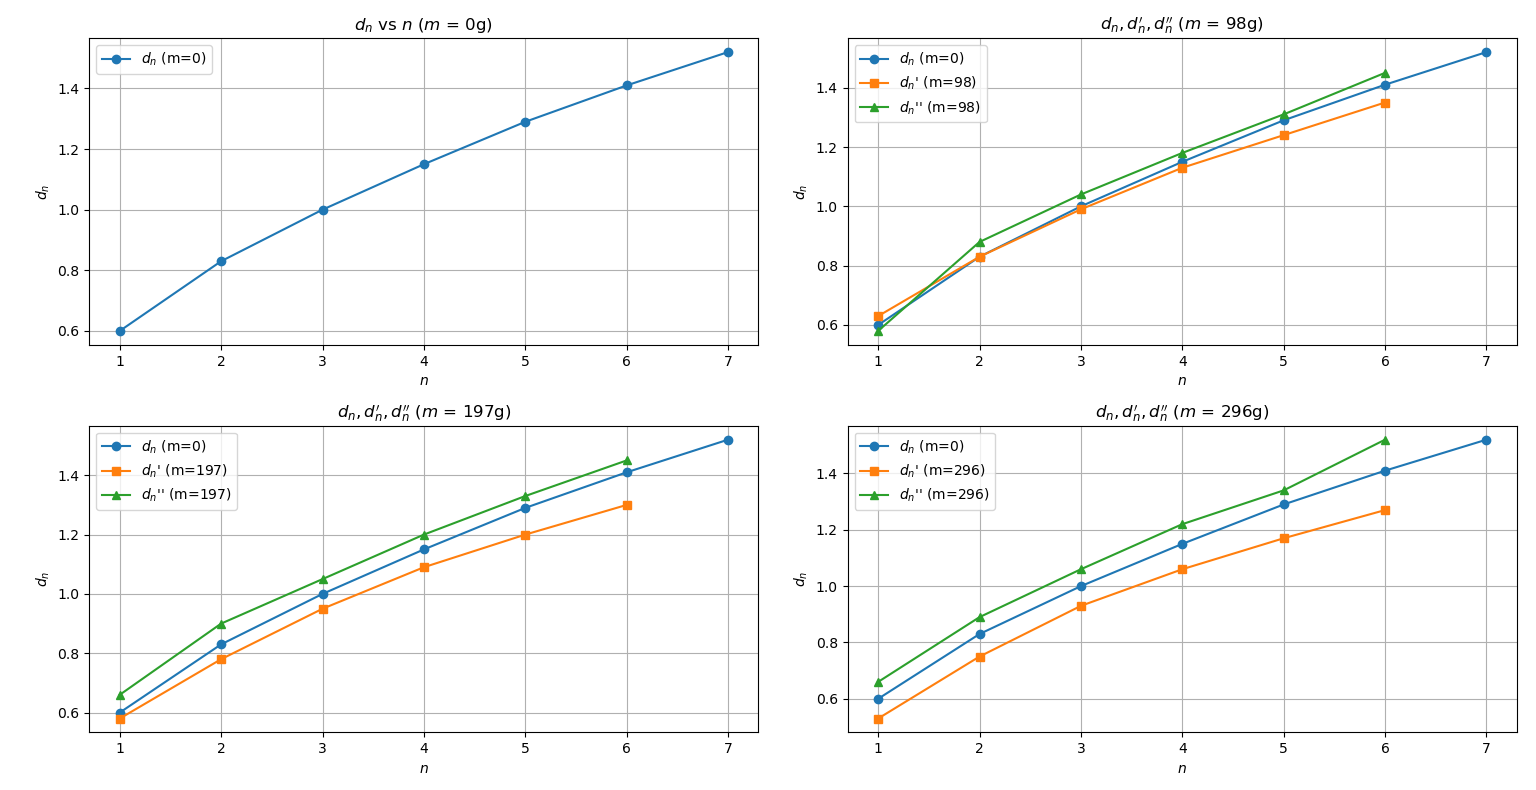
\includegraphics[width=1\linewidth]{4diff}
	\caption{Plot of Talble 1 - 4 with $d_n$ to compare}
\end{center}
From this we see that other than Table - 2 (Top right figure) every other plots seems fine. In the Table two, thhr Hence in our later calcualtiosn we will not consider data from Table - 2 (The general expected order should be $d_n'' > d_n > d_n'r$ but we dont see it for the inital values). 

Now using Table - 1 and Equation - 8 for uncertainty, we plot $n$ vs $d_n^2$ as: 
\begin{center}
	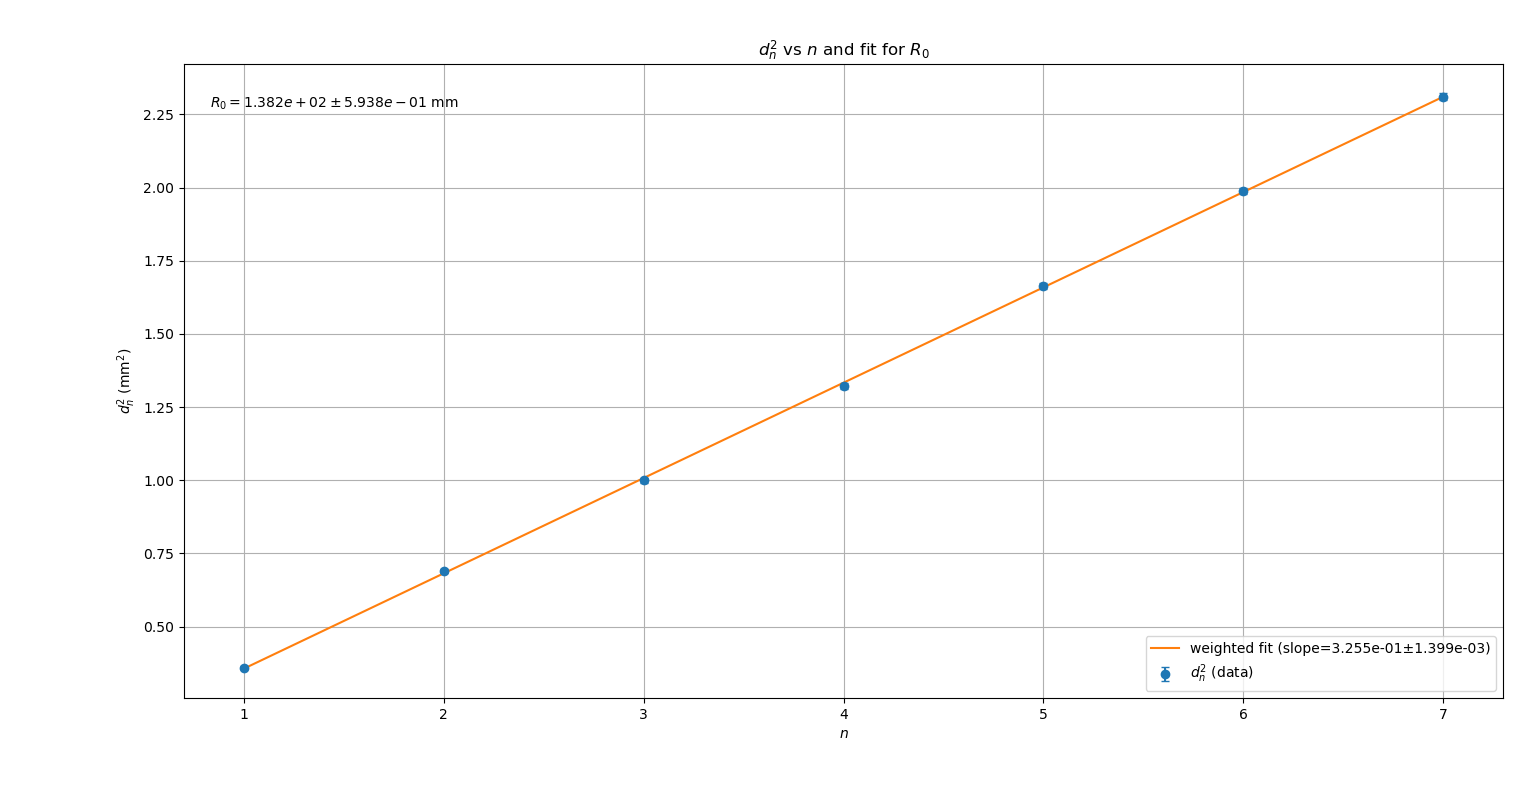
\includegraphics[width=1\linewidth]{R0}
	\caption{Linear best fit with error to calculate $R_0$}
\end{center}
Now to calcualte the $R_1$ and $R_2$ we use the Equation 4, 5 to calculate it and Equation 10, 11 for its error. Doing it we get:
\end{figure}
\begin{figure}[H]
        \centering
	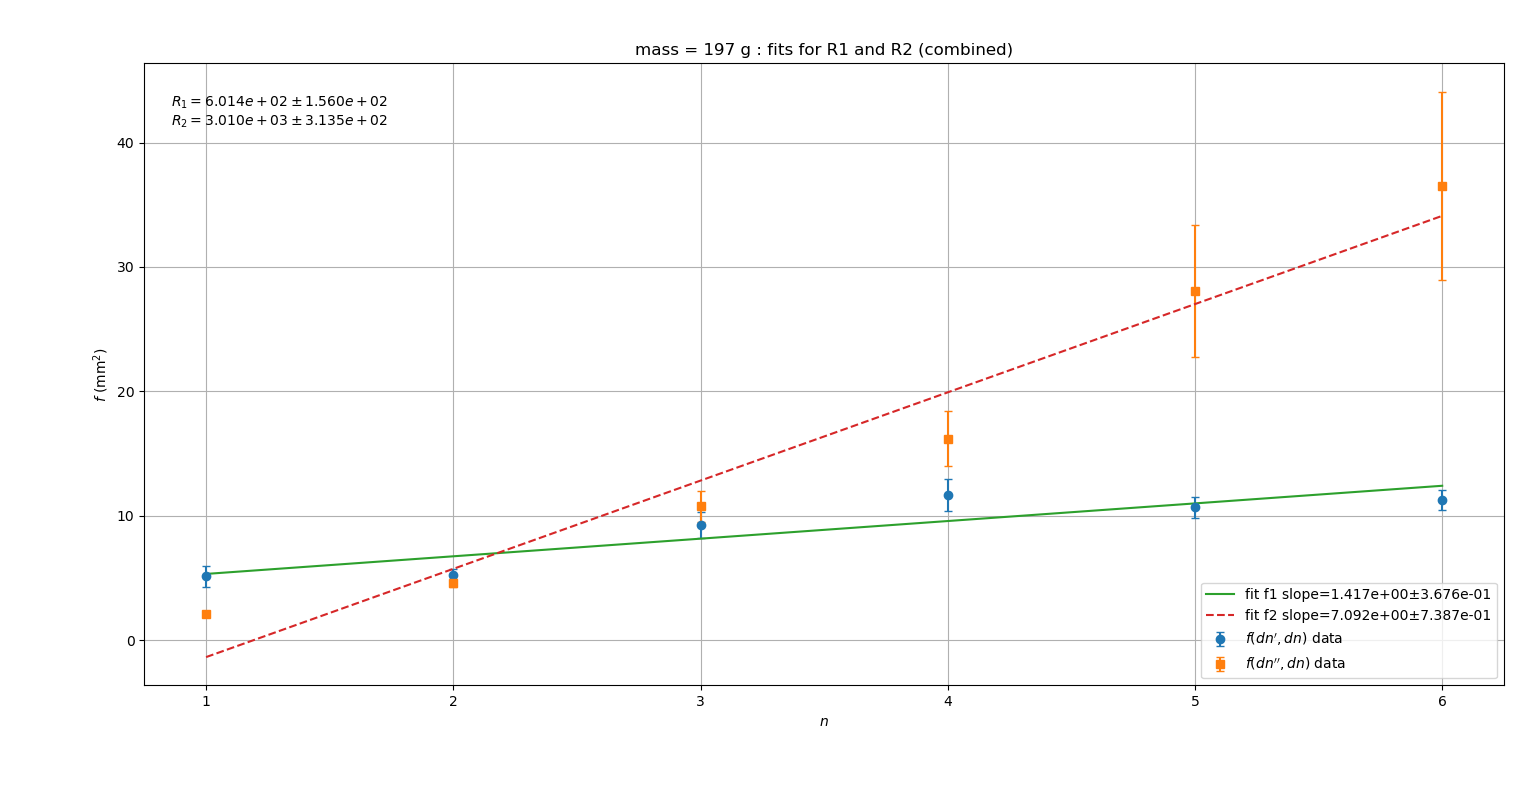
\includegraphics[width=1\linewidth]{197}
		\caption{Plot for $m_1$ = 197g  to calculate $R_1$ and $R_2$}
        \centering
	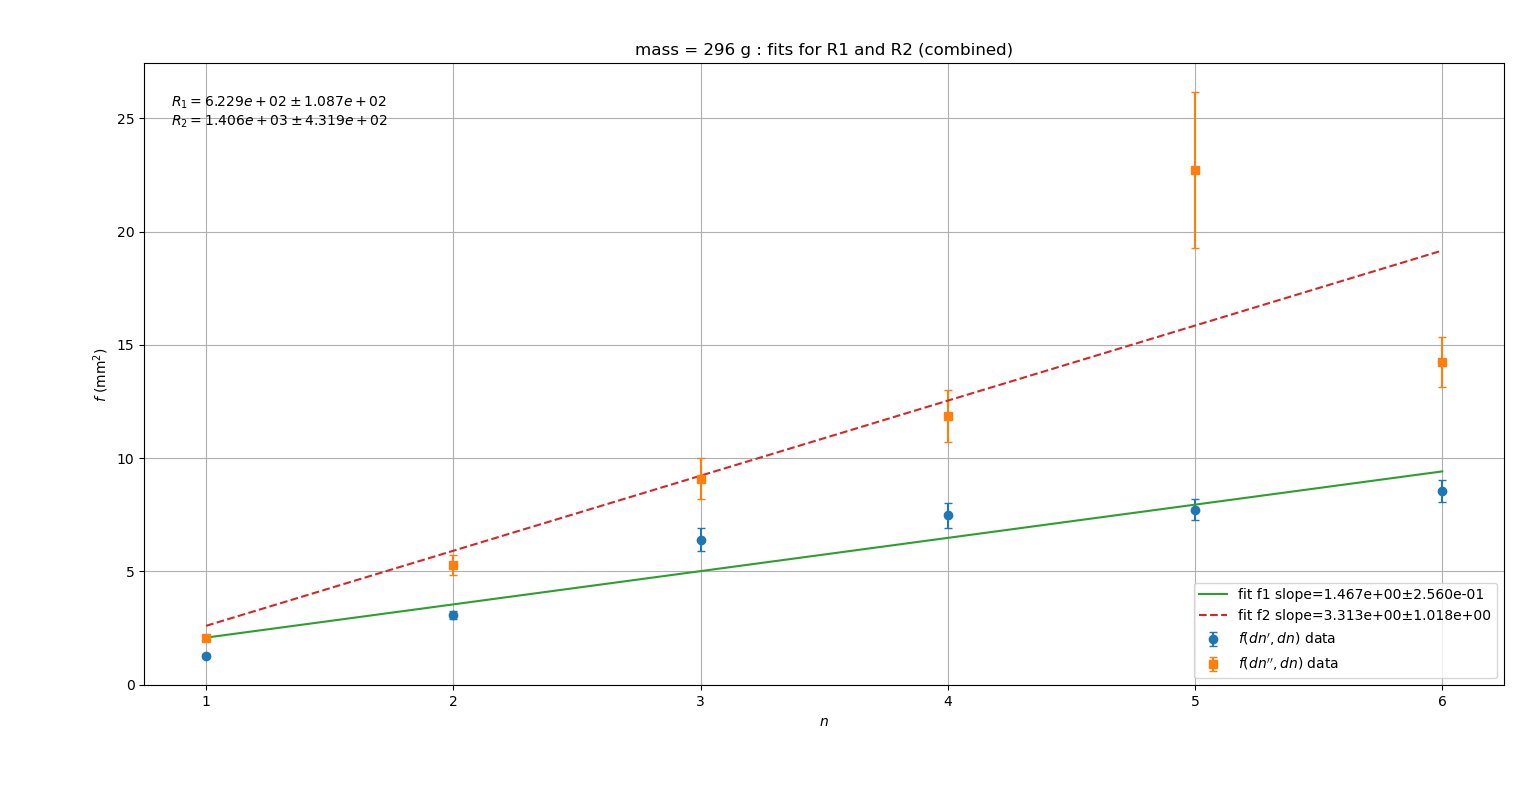
\includegraphics[width=1\linewidth]{296}
		\caption{Plot for $m_1$ = 296g to calculate $R_1$ and $R_2$}
\end{figure}
From FIG. 6 and 7, we see that the calculated value of $Y$ and $\zeta$ for each mass. Doing a weighted sum we get, $Y =  1.05145*10^9 \pm   3.23540* 10^8$ \si{\gram\per\second\per\mm\squared}.
\section{Result and Conclusion}
Hence after converting to SI, the Young's modulus will have unit of Pascals and Possion's ratio will be unitless. The final values we get are:
\begin{empheq}[box=\fbox]{align*}
\text{Young's modulus }(Y) &= 1.0 \pm 0.3 \text{ \si{\giga\pascal}}\\ 
\text{Poisson ratio }(\mu) &= 0.325 \pm 0.17
\end{empheq}
The error in these values along with the theoretical value will be discussed in Appendix A.
\vspace{0.6cm}
\hrule
\hfill \pagebreak

\bibliographystyle{apsrev4-2}
\bibliography{refrences}


\appendix
\section{Theoretical values and Uncertainty}
Perspex (PMMA) acrylic typically exhibits a Young's modulus of 2.4–3.3 GPa (2400–3300 MPa) and a Poisson's ratio of 0.35–0.4. The cause of the deviation for Young's modulus is attributed to very small sample of masses taken. The Possion's ratio fits well within the theoretical value although it has very high uncertainty again because of low sample size.

\section{Imporovments in procedure}
The uncertainty can be decreased by taking more weight measurements. Furthermore to reduce human error we can take multiple measurements for each mass. We can also reduce some systematic errors, such as the weight of the slab, by measuring it and taking it into account for calculations. To have correct fringe index, we can take a picture to determine the peaks, this will be more accurate than eye and can also be double checked later.

\end{document}
